%%%%%%%%%%%%%%%%%%%%%%%%%%%%%%%%%%%%%%%%%
% "ModernCV" CV and Cover Letter
% LaTeX Template
% Version 1.11 (19/6/14)
%
% This template has been downloaded from:
% http://www.LaTeXTemplates.com
%
% Original author:
% Xavier Danaux (xdanaux@gmail.com)
%
% License:
% CC BY-NC-SA 3.0 (http://creativecommons.org/licenses/by-nc-sa/3.0/)
%
% Important note:
% This template requires the moderncv.cls and .sty files to be in the same
% directory as this .tex file. These files provide the resume style and themes
% used for structuring the document.
%
%%%%%%%%%%%%%%%%%%%%%%%%%%%%%%%%%%%%%%%%%

%----------------------------------------------------------------------------------------
%	PACKAGES AND OTHER DOCUMENT CONFIGURATIONS
%----------------------------------------------------------------------------------------

\documentclass[12pt,a4paper,sans]{moderncv} % Font sizes: 10, 11, or 12; paper sizes: a4paper, letterpaper, a5paper, legalpaper, executivepaper or landscape; font families: sans or roman

\moderncvstyle{casual} % CV theme - options include: 'casual' (default), 'classic', 'oldstyle' and 'banking'
\moderncvcolor{purple} % CV color - options include: 'blue' (default), 'orange', 'green', 'red', 'purple', 'grey' and 'black'

\usepackage{lipsum} % Used for inserting dummy 'Lorem ipsum' text into the template
\usepackage[scale=0.75]{geometry} % Reduce document margins

\setlength{\hintscolumnwidth}{3cm} % Uncomment to change the width of the dates column

% \setlength{\makecvtitlenamewidth}{8cm} % For the 'classic' style, uncomment to adjust the width of the space allocated to your name

%----------------------------------------------------------------------------------------
%	NAME AND CONTACT INFORMATION SECTION
%----------------------------------------------------------------------------------------
\usepackage{xcolor}
\definecolor{bleudefrance}{rgb}{0.19, 0.55, 0.91}
\firstname{\textcolor{bleudefrance}{Soumya}}
\familyname{\textcolor{cyan}{Prasad}}

% All information in this block is optional, comment out any lines you don't need
\title{Experienced test engineer}
\address{Söderberga Allé 52}{16862, Bromma}
\mobile{+46 73 340 1229}
\email{soumya.saligram@gmail.com}
\social[linkedin][https://www.linkedin.com/in/soumyaprasad/]{Soumya Prasad}
\social[github]{chisma}


\photo[60pt][0.8pt]{pictures/picture} % The first bracket is the picture height, the second is the thickness of the frame around the picture (0pt for no frame)
%\textcolor{cyan}{\fboxrule=3pt\fbox{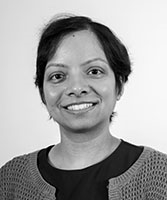
\includegraphics[height=1.3in]{pictures/picture}}}

%----------------------------------------------------------------------------------------

\begin{document}
\makecvtitle


\section{Summary}
I am an engineer, with several years of experience within various areas of product testing. I enjoy automating tests, and in the process,
refine the product and its value, always, with the end user in focus. Continuously collaborating with developers, product owners,
account managers and testers - to best align with the use-case, while at the same time maintaining a high code coverage , are my strengths.

\hfill \break
I have been working as a test developer at {\href{https://www.cinnober.com/}{\color{cyan}Cinnober Financial Technology}} since September 2017. I work
in a project for {\href{https://www.jse.co.za/}{{\color{cyan}Johannesburg Stock Exchange}}. In my day job, I write functional tests for newly added features and bug fixes in a JUnit - based framework. I also work with CI:
deployment, monitoring and troubleshooting.


\hfill \break
Business point of view, I am familiar with post trade solutions and
trading platforms in general(With hands-on knowledge of clearing technology for stock exchanges). I have also briefly worked
with IoT sensor networks and for several years in industrial automation.

\hfill \break
I am looking for testing roles involving API/Backend testing of Java based services or products. I am easy to work with,
a keen learner, very communicative and thrive working in a team. Recently, I am reading up about cloud technologies/BigData/ML
and find them exciting. I can communicate in English and Swedish.


\section{Experience}
\cventry{Sep, '17 - current}{Test Developer}{\href{https://www.cinnober.com/}{\textsc{\color{cyan}Cinnober(Part of Nasdaq)}}}{Stockholm}{}{
\begin{itemize}
\item Writing functional tests for REST APIs
\item Collaborate with developers in the team, for bug fixes or tasks to be automated
for the current release and/or patch delivery
\item Have the tests integrated to CI pipeline/s for various work flows, as soon as possible.
\item Daily monitoring of CI builds for breakages, flaky tests.
\item Troubleshooting, debugging of CI bottlenecks and failures from the build log files
\item Writing scripts to enable quick retrieval of data from CI builds- for generating client reports
\item Update, track backlog on JIRA.
\item Act as scrum master for testing sprints
\item Drive well documented code, commits, tests and requirements
\item Drive consistent good performance on code quality jobs on CI
\item JavaSE8, Eclipse, JUnit4, SmartGit, Python3, Confluence, JIRA, SonarCube
\end{itemize}
}


\cventry{May '17 - July '17}{Intern}{\href{https://www.yanzi.se}{\textsc{\color{cyan}Yanzi}}}{Stockholm}{}{
\begin{itemize}
\item Testing of a websocket based REST API with Mocha/Chai libraries
\item Documenting the API using LaTeX, in a unix environment.
\item JavaScript
\item Mocha/Chai/BDD
\item REST API/websockets
\item LaTeX
\end{itemize}
}


\iffalse
\section{Training}
\cventry{Feb, '17 - June '17'}{Student}{\textsc{\color{cyan}Lexicon IT Konsult}}{Stockholm}{}{
	\begin{itemize}
	\item JavaSE8
	\item JavaEE fundamentals
	\item Spring/Hibernate fundamentals
	\item Maven fundamentals
	\item JUnit
	\item SQL fundamentals
	\item HTML5/CSS/JavaScript
	\item Eclipse IDE on Linux/Windows
 	\end{itemize}
  }
\fi

%\section{Experience}
\cventry{Apr,12 - May,13}{Associate lead}{\href{https://www.se.com/se/en/}{\textsc{\color{cyan}Schneider Electric}}}{Bangalore}{}{
    \begin{itemize}
    \item Worked closely with development teams and different stakeholders in an agile environment (daily standup, sprints, retrospectives, continuous integration).
    \item Worked on improving test automation with TestComplete.
    \item Created development tasks from user stories.
    \item Used project management tools such as Assembla, TestComplete 9.0, Git (on Windows), Beyond Compare at various stages of test automation life cycle.
    \item Worked closely with various teams during user acceptance and release.
    \end{itemize}
}

\cventry{Dec,05 - Mar,12}{Senior engineer}{\href{https://www.honeywell.com}{\textsc{\color{cyan}Honeywell}}}{Bangalore}{}{
    \begin{itemize}
    \item Define test plans and test specifications for integration, functional and performance testing, execution of test cases.
    \item Performance benchmarking using perfmon of an SQL server based application. This included test bed setup, designing test data, and deriving non functional requirements.
    \item Continuously worked to evolve new strategies for test automation.
    \item Implemented hardware virtualization using VMWare.
    \item Root cause analysis and continuous process improvement(Kaizen).
    \item Set up the processes required to promote the overall quality of the product.
    \end{itemize}
}

\cventry{Nov,03 - Nov,05}{Project engineer}{\href{https://www.ge.com/in/intelligent-platforms}{\textsc{\color{cyan}GE India}}}{Bangalore}{}{
    \begin{itemize}
    \item Study the design and technical specifications received from customer and understand the process requirements and deliverables.
    \item Develop the main PLC logic using the Ladder language and VB scripting.
    \item Participate in customer interactions, project reviews and software inspection.
    \end{itemize}
}

\section{Education}
\cventry{Feb, '17 - June '17'}{Trainee}{\href{https://www.lexicon.se/IT-Proffs/IT-Proffs/Oversikt/}{\textsc{\color{cyan}Lexicon IT Konsult}}}{Stockholm}{}{
	\begin{itemize}
	\item JavaSE8
	\item JavaEE fundamentals
	\item Spring/Hibernate fundamentals
	\item Maven fundamentals
	\item JUnit
	\item SQL fundamentals
	\item HTML5/CSS/JavaScript
	\item Eclipse IDE on Linux/Windows
 	\end{itemize}
  }

\cventry{1999--2003}{\textsc{Bachelor of engineering}}{\href{http://vtu.ac.in/en/}{\textsc{\color{cyan}VTU}}}{Bangalore}{}{Specialized in instrumentation technology with consistently good academic record}

\section{Awards}

\cvitem{2009}{Bravo-Gold:Process Excellence, Honeywell}
\cvitem{2007}{ACS Special Award, Honeywell}
\cvitem{2006}{Team excellence award, Honeywell}

\end{document}
